\section{Discussion}
\label{sec:disc}


%%%
% Discussion
%%%

%%%
This thesis focused on an attempt to use
$\epsilon$-greedy Monte Carlo methods with exploring starts
to develop a well-playing
cribbage agent capable of weighing different strategies
with the intention of using these learned weights to 
potentially
improve the play of the author and readers.
%
In the primary objective of evolving a cribbage agent to a good strategy,
despite the setbacks of poor performance on a per-game level,
the agent did remarkably well
by removing irrelevant strategies
such as \handmaxmed\ and \peggingmaxmedgained\ 
and emphasizing more useful strategies
like \handmaxavg\ and \handmaxmin.
%%%

%%%
This section will describe some reasons for successes and failures of the learning
process as well as potential future applications or improvements to the
system which can help make a successful cribbage-playing agent in the future.
%%%

% Discussion of Future possibilities for thesis topic/area

\subsection{Future Possibilities}
\label{sec:disc-future}

%%%
Due to assumptions and simplifications
made throughout the design and implementation process,
several suboptimalities exist across this thesis
which leave room for improvement for future endeavors to solve the task
of learning to play cribbage well.
%%%

% Pegging future work

\subsubsection*{Pegging}
\label{sec:disc-future-pegging}

%%%
% Discussion of what can be done for learning pegging better
% Shortcomings:
%	1. only a basic heuristic
%		- can train a player for this alone
%	2. estimate performance on incomplete/small amount of data
%		- pre-populated a bit, but ~50-100k, not millions
%			(definitely missing some combos when first round started)
%%%

%%%
% Basic intro paragraph*
%%%

%%%
One area of the project that can be improved was the pegging system.
%
Because the focus of the thesis was on whether or not a collection of
strategies could be learned in combination when choosing which cards to keep,
an ideally playing agent was not the outcome.
%
A key reason for this was the lack of time dedicated to and nonchalant nature
towards learning how to actually play the crucial pegging phase.
%%%

\paragraph*{Playing Strategy}

%%%
% Discussion of Failures of basic heuristic
%	- very basic strategy only looks one immediate step ahead
%	- no context awareness as to whether to play offensively/defensively
%		(ironic)
%%%

%%%
The first shortcoming of the pegging portion of the agent was the simplicity
of its playing strategy.
%
In order to focus on the overall playing strategy and to have a consistent
knowledge of how a set of cards have performed in the past,
the agent was only capable of following a very simple immediately greedy 
heuristic:
of the cards available which are legal to play,
play the one with the highest immediate return.
%
This has the potential flaw of
opening oneself up to the possibility of allowing the opponent an opportunity
to score more than the agent itself just gained,
resulting in a net loss.
%
As has been demonstrated by the rest of this thesis,
the idea that one strategy can be applied at all times in the game of cribbage
is laughable.
%so the single heuristic used is 
%%%

%%%
In future applications,
a partial agent could be trained in just the pegging phase alone
using reinforcement learning.
%
In a similar way to this thesis,
multiple basic strategies such as offensive or defensive play
could be trained by rewarding each behavior and their combinations
could in turn be learned through gameplay simulations.
%
Alternatively,
a more ground-up approach can be taken to train an unbiased agent by simply
having each player learn from trial and error with certain card combinations.
%
%This has the disadvantage of taking more time to train to effectiveness.
%
In either case,
a more suitable pegging system can be made that would play better.
%%%

\paragraph*{Performance Evaluation}

%%%
Even though a better pegging system can be made,
key to this thesis was the idea that performance can at least be
anticipated with some amount of certainty.
%
In this project,
the performance of the pegging agent was tracked by card combination,
recording the points scored and yielded during each occurrence.
%
These records were used to anticipate how each combination of cards would
play against an opponent.
%%%

%%%
Before the first round of training,
however,
there was relatively little pre-population of these records done:
roughly one hundred thousand randomly dealt hands were played against each
other.
%
As a result of the small sample size,
performance estimates were likely to be inaccurate.
%
Furthermore,
the small sample size did not cover all of the possible hand
combinations.
%
Because of this,
data would be missing for multiple combinations of cards
for the decision process
throughout the first round.
%
This means that the card combinations' true desirability would be
misrepresented during the calculation,
allowing for the possibility of an unfair
punishment or reward for what would amount to a guess by the
pegging-based strategies.
%
It also means that the information received by the agent during the weighting
operation would not be static, with respect to the cards given,
as other strategies were and thus could not be as
reliably trusted for accuracy.
%
While
this was counteracted by using records from a first round training session in 
all subsequent training sessions,
the concern remains whether this was enough
and how much the variability in the data provided by the pegging strategies
affected learning.
%%%




\subsubsection{Implementation Decisions}
\label{sec:disc-future-implementation}

%%%
Because of the author's previous experience in only small-scale uses for
cribbage software,
experience with optimizing software for large-scale computation tasks was
lacking.
%
This inexperience,
in combination with the desire to develop a prototype quickly
in a familiar environment,
led to the decision to write the majority of this thesis in Python.
%
This,
to put it bluntly,
was a mistake because of the unforeseen complications and side effects
that that decision led to.
%%%


\paragraph{Database Dependency}

%%%
Because Python was the language of choice,
the performance of making a decision for a single hand was abysmal:
on a development machine,
the decision for a single hand would take approximately ten seconds,
%
As previously mentioned in the Methods section,
the decision made from that point was to create a database such that all
calculations were done ahead of time
and the statistics desired would be available upon request.
%
This succeeded in its desired goal,
bringing the time required for a single decision to approximately
one twentieth of a second.
%
At this point the project was able to play two games in about a second's time
on the same development machine.
%%%

%%%
Despite the speed improvements in a development environment,
now the entire training process had become I/O-bound rather
than CPU bound.
%
In and of itself,
this was not a problem until an attempt was made to train multiple
agents simultaneously.
%
Because of concurrency issues which would have,
if even possible,
taken too long to fix,
no more than one process could successfully access the database with any
consistency.
%
This would mean that only two agents could be trained on each database at any
given time.
%
Furthermore,
since this database file was around twenty gigabytes in size and
there was only limited local storage space available
on each of the compute nodes in the Computer Science Department's high
performance compute cluster,
jobs had to be constructed carefully and spread across nodes to avoid
accidentally disrupting other users' calculations.
%%%

%%%
Were this project to be repeated,
it would be recommended to use the Python code from this attempt as an outline
for a rewrite in a slightly lower-level language.
%
Using a language such as C++,
which could be optimized more for run-time efficiency and memory management,
would likely increase speed of computation enough to remove the necessity
of a statistics database entirely.
%
While the data gathered from previously played pegging rounds would still need
to be stored and retrieved between training rounds,
the size of this data would likely not exceed a few gigabytes and would fit
easily in the program's RAM space.
%
This is especially true since the strategies utilizing the median were not
learned to be a useful metric for choosing cards,
meaning that a list of scores gained and given are not needed,
only the cumulative amount and times seen.
% TODO: ^^^ ensure accuracy
%
Also,
like weight checkpoints are in the current system,
these stored results could be exported in a text or otherwise simple format
for transfer between rounds.
%%%

%%%
With these changes made,
the training program would be CPU-bound,
which thankfully can be countered by adding or improving hardware.
%
In contrast,
the I/O-bound training program used in this thesis used only half the total
processing power of a single CPU core
as the limitation was the database file on a solid state drive.
%%%




%%%
% how the linearity of input/policy affected outcome
%%%



%% Discussion of how we learned policy which didn't have enough information
% and how value function improvement would have been better

\subsection{Learning Policy vs. State-Value Function}
\label{sec:disc-value}

%%%
This thesis focused on an attempt to use Monte Carlo-based value iteration
to develop a well-playing
cribbage agent capable of weighing different strategies
with the intention of using these learned weights to 
potentially
improve the play of the author and readers.
%
In the primary objective of evolving a cribbage agent to a good strategy,
despite the setbacks of poor performance on a per-game level,
the agent did remarkably well
by removing irrelevant strategies
such as \handmaxmed\ and \peggingmaxmedgained\ 
and emphasizing more useful strategies
like \handmaxavg\ and \handmaxmin.
%%%

%%%
One of the reasons for its poor per-game play
is the lack of knowledge as to how a set of cards lends itself to being played
with a certain strategy.
%
The extent to which the cards themselves affect the action choice in the policy
was greatly underestimated.
%
However,
to include the knowledge of which cards are known into the policy decision
would have increased the dimensionality of the search space from the relatively
small three-dimensional problem tackled to a problem of at least nine
dimensions,
depending on the cards' encoding method.
%
At this dimensionality,
the search space would be far too massive and sparse to simulate an amount of
games which would lead to any worthwhile learning
in a manageable amount of time.
%%%

%%%
An alternative to including the cards in the policy would be to not
directly use a policy at all.
%
Instead,
the state-value function could be used,
as done with TD-Gammon~\cite{tdgammon},
AlphaGo~\cite{deepmind_alphago,deepmind_alphago_zero},
and O'Connor's senior project~\cite{roconnor_cs486}.
%
By learning the state-value function instead of a policy,
an agent could determine which set of cards would likely place itself in the
most optimal resulting position,
indirectly developing its own policy.
%
This form of value iteration should allow for a more adaptive agent
and thus more optimal gameplay,
leading to an agent that might win more consistently.
%%%

%\input{sections/discussion/value/*}


%%%
% Discussion on how the model's setup may have led down path to "failure"
%%%

\subsection{Shortcomings of the Model}
\label{sec:disc-shortcomings}

%%%
In addition to the shortcomings of the implementation decisions made or
necessitated by other decisions,
the features of the model itself should be considered and evaluated.
%
Several assumptions were made to limit the scope and dimensionality of the
problem,
but it is likely the case that these limitations also affected the
potential learning ability of the agent.
%%%


\subsubsection*{Linearity}
\label{sec:disc-shortcomings-linearity}

%%%
% How the linearity of the model may be responsible for poor play
%%%

%%%
One of the model's shortcomings that must be addressed is the linearity
of the decision making apparatus.
%
As described in Section~\ref{sec:dm-methods-weighting},
the mechanism for deciding which combination of cards to choose is,
at its core,
a simple linear operation.
%
The weights vector $\wvecm_{p,o,d}$ is multiplied by a desirability matrix \Smat\
to produce a probability vector \pvec,
from which the maximum value is chosen when the policy is strictly followed.
%
Although a human player would indeed evaluate which combinations are best
to play with a set of strategies with varying importance over the course
of the game,
the nature of this relationship in the player's mind is unlikely
to be a simple linear function.
%
Instead,
a human player would also consider how two or more strategies would interact
with each other at different points in the game.
%%%




\subsubsection*{Strategies}
\label{sec:disc-shortcomings-strategies}

%%%
% How the limited number of strategies themselves may have contributed
%%%

%%%
Another shortcoming of the setup to the model to the problem of this thesis is
the limitation of the strategies chosen.
%
Since each strategy's contribution to the \Smat\ matrix can be thought of as
a feature,
this means that the final model is no more than a simple linear combination of
eight features
used to determine the best choice of cards.
%used to predict the outcome of a card-game.
%
Furthermore,
the features selected,
although sensibly selected by a fairly experienced cribbage player,
may themselves not be ideally suited to the task at hand.
%%%


%%%
% Approach the idea of neural network solution
%%%

%%%
As a result of these previous shortcomings,
a better solution for the future would be to use an architecture that allows
for the learning of nonlinearities and automatic feature discovery and
learning,
such as a neural network
as per ~\cite{deepmind_alphago} and ~\cite{tdgammon}.
%%%



%%%
% How the results given can be of use to a future project
% despite shortcomings
%%%

\subsection{Usefulness of Results}

%%%
% Intro paragraph
%%%

%%%
Despite the final learned agent's shortcomings in ability to consistently win
a single game,
the deliverables of this project can still be applied to expand the current
knowledge of cribbage as well as serve as a guidance story.
%
As they were intended from the outset,
the generated strategy graphs can serve as a set of guidelines as to how a
player ``should'' be playing a certain hand.
%
Although a human player may not be able to calculate the statistics which the
agent used as accurately as a computer,
a fair amount of experience and intuition can be gained through repeated
play which should approximate the expected and guaranteed returns well.
%%%

%%%
The agent's successes in the macro scale can also be of use to those
applications which also operate on the scale of thousands to millions of games.
%
Mainly,
the developed agent could be used for a first round or two of training
of a value-function based agent.
%
Rather than learning from the self-play with no existing knowledge,
a policy-following agent can be played against instead.
%
Playing an agent of greater difficulty would allow the value function optimizing
agent to more quickly converge to an optimum.
%
Since the results of this thesis were achieved without imparting any particular 
pre-existing domain knowledge to the initial policy,
this faster convergence to optimal would not be unfairly biased
towards any form of human play,
thus lowering training time without introducing suboptimalities.
%%%


% Figures

\begin{figure}
\center
\begin{subfigure}[b]{0.66\textwidth}
	\center
	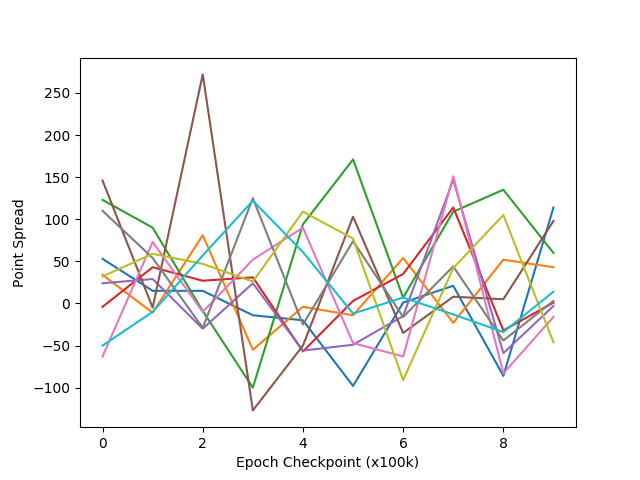
\includegraphics[height=0.22\textheight]{images/discussion/usefulness/r2-time-series-9.png}
	\caption{Point spreads for 9-game matches, like in human play.}
	\label{r2-time-series-9}
\end{subfigure}
~
\begin{subfigure}[b]{0.66\textwidth}
	\center
	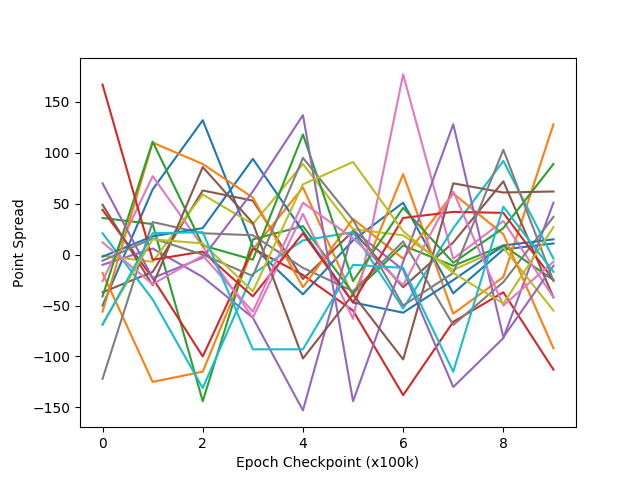
\includegraphics[height=0.22\textheight]{images/discussion/usefulness/r2-time-series-100.png}
	\caption{Point spreads for 100-game matches.}
	\label{r2-time-series-100}
	% TODO: ^^^ make sure we have an accurate graph,
	%		scale leads me to believe we have the wrong graph
\end{subfigure}

\begin{subfigure}[b]{0.66\textwidth}
	\center
	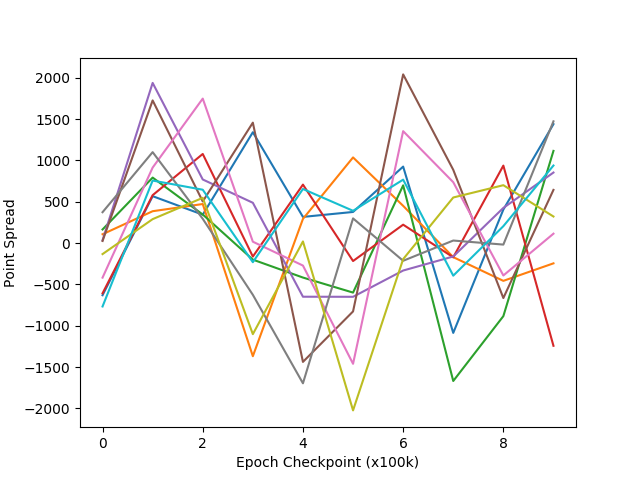
\includegraphics[height=0.22\textheight]{images/discussion/usefulness/r2-time-series-1000.png}
	\caption{Point spreads for 1,000-game matches.}
	\label{r2-time-series-1000}
\end{subfigure}
~
\begin{subfigure}[b]{0.66\textwidth}
	\center
	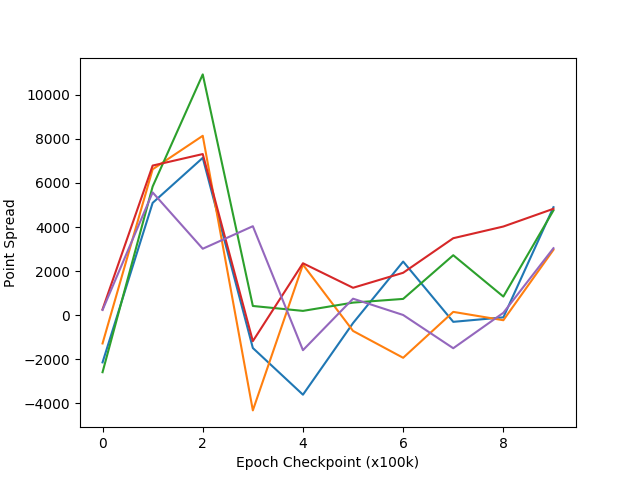
\includegraphics[height=0.22\textheight]{images/discussion/usefulness/r2-time-series-10000.png}
	\caption{Point spreads for 10,000-game matches.}
	\label{r2-time-series-10000}
\end{subfigure}

\caption{
	Point spreads across matches of varying lengths.
	In each graph,
	the final \learned\ agent is played against its previous checkpoint
	iterations.
}
\label{fig:r2-time-series}
\end{figure}

% /Figures


%%%
% Discussion of how scale affects score spreads
%	On 9-game scale, we have utter chaos, maybe not worth mentioning?
%	On 100-game scale, utter chaos
%	On 1000-game scale, maybe a little, if we squint hard,
%	On 10k-game scale, we can see a pattern
%		contradicts the 1k-game observations
%		consistently even with random
%		sharp increase in performance over 100k-200k
%		even play for the next 600k
%		seemingly regain advantage in the last 200k
%%%

%%%
A regulation cribbage match between two human players consists of nine games.
%
As can be seen in Figure~\ref{fig:r2-time-series-100},
in a series of 100-game matches between a fully trained agent and its
previous checkpoints,
no pattern is discernible in total point spreads between the two playing agents.
%
This demonstrates that,
on this scale,
the winner of the game is no more predictable than a truly random coin toss.
%%%

%%%
When the scale is increased to one thousand games,
a slight pattern begins to emerge
when visualized in Figure~\ref{fig:r2-time-series-1000}
%
Whereas the majority of the graph remains highly varying and unpatterned,
the first few games follow a common pattern.
%
The match against the random agent is still unpredictable,
but the matches against the 100,000 and 200,000 game trained checkpoints are
consistently beaten by the final agent.
%%%

%%%
Although fewer matches are played to accommodate the increased time needed to
play the increased number of games,
the same pattern present in the thousand-game scale is visible in the
ten thousand-game matches.
%
With the exception of the purely untrained agent,
the least \learned\ agents perform the poorest against the final
\learned\ agent.
%
Play are approximately evenly matched when between agents
when the opposing agent has trained for 300,000 to 700,000 games.
%
Following these matches,
the agent begins to again win more consistently when more training is done.
%%%

%%%
If the agent is being trained correctly and no overfitting is occurring,
then the point spread should be a positive number,
gradually decreasing and approaching zero
as more training is applied to its opponent,
forming a similar curve to a loss metric used in classical machine learning.
%
In the event of overfitting,
the curve would dip below the zero before reapproaching zero.
%
Neither of these shapes were seen in the resulting graph
(see Figure~\ref{r2-time-series-10000}).
%
Instead,
the shape of the curve implies that,
since the random agent performs consistently better than the trained agent,
the learning process is not learning the game so much as how to outplay its
opponent.
%
This conclusion is supported by the observation that the agents with limited
training are steadfastly outplayed.
%%%

%%%
However,
since there is a sharp dip after 300,000 training epochs before increasing
again,
the results are difficult to interpret.
%
The final \learned\ agent is more evenly matched in performance with an agent
trained for 400,000 games
than it is against a more recently trained agent.
%
The reintroduction of an increasing curve
is an indicator of overfitting in the middle stages.
%
Whereas the final agent is able to play well against these agents,
they themselves have decreased in performance capability.
%
This is speculated to be a result of learning how to outplay its opposing agent
rather than an understanding of the game.
%
This is contingent upon the results of the round-robin play though,
so no conclusions can be drawn at this time.
% TODO ^^^ reaffirm when round-robin play is completed
%%%

%%%
Also of further note is the scale on the aforementioned graphs.
%
In Figure~\ref{r2-time-series-10000},
the maximum point spread achieved is just a shade above 10,000 points
over the course of 10,000 games.
%
This means that the average point spread advantage is approximately 
one point per game at peak performance\textemdash
and most often $0.2$ points per game\textemdash
in long-term play.
%
The average spread increases to $25$ points per game when fewer games are 
played,
but since performance is unpredictable on this scale,
this can be explained as a result of the randomness of the cards given
and cannot be considered a reliable measure of performance.
%
In fact,
in sampled matches,
it was not uncommon to observe losses and wins of 30 points or more
as well as much closer games with margins of only a few points.
%
In addition to the randomness of cards dealt,
this massive point sway could also be the result of the agents' uncertainty on 
how to recover from a losing position.
%
While the reasons for this inability cannot be said to be more than speculation,
the learning of a policy directly without taking into account cards dealt
is the likely culprit,
as explained previously.
%%%



%\input{sections/discussion/usefulness/*}


